% Created by tikzDevice version 0.12.3.1 on 2021-04-14 21:08:23
% !TEX encoding = UTF-8 Unicode
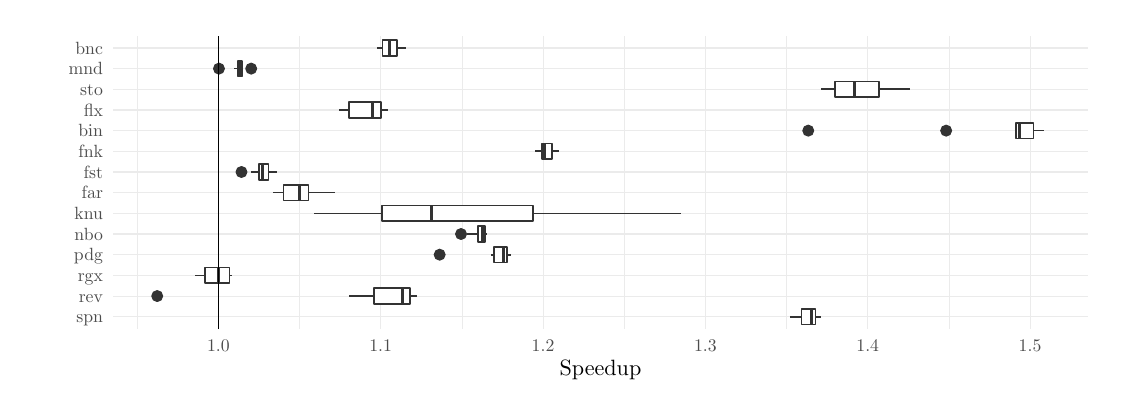
\begin{tikzpicture}[x=1pt,y=1pt]
\definecolor{fillColor}{RGB}{255,255,255}
\path[use as bounding box,fill=fillColor,fill opacity=0.00] (0,0) rectangle (390.26,130.09);
\begin{scope}
\path[clip] ( 30.80, 21.16) rectangle (383.14,127.24);
\definecolor{drawColor}{gray}{0.92}

\path[draw=drawColor,line width= 0.2pt,line join=round] ( 39.57, 21.16) --
	( 39.57,127.24);

\path[draw=drawColor,line width= 0.2pt,line join=round] ( 98.23, 21.16) --
	( 98.23,127.24);

\path[draw=drawColor,line width= 0.2pt,line join=round] (156.90, 21.16) --
	(156.90,127.24);

\path[draw=drawColor,line width= 0.2pt,line join=round] (215.56, 21.16) --
	(215.56,127.24);

\path[draw=drawColor,line width= 0.2pt,line join=round] (274.22, 21.16) --
	(274.22,127.24);

\path[draw=drawColor,line width= 0.2pt,line join=round] (332.88, 21.16) --
	(332.88,127.24);

\path[draw=drawColor,line width= 0.4pt,line join=round] ( 30.80, 25.64) --
	(383.14, 25.64);

\path[draw=drawColor,line width= 0.4pt,line join=round] ( 30.80, 33.11) --
	(383.14, 33.11);

\path[draw=drawColor,line width= 0.4pt,line join=round] ( 30.80, 40.59) --
	(383.14, 40.59);

\path[draw=drawColor,line width= 0.4pt,line join=round] ( 30.80, 48.06) --
	(383.14, 48.06);

\path[draw=drawColor,line width= 0.4pt,line join=round] ( 30.80, 55.53) --
	(383.14, 55.53);

\path[draw=drawColor,line width= 0.4pt,line join=round] ( 30.80, 63.00) --
	(383.14, 63.00);

\path[draw=drawColor,line width= 0.4pt,line join=round] ( 30.80, 70.47) --
	(383.14, 70.47);

\path[draw=drawColor,line width= 0.4pt,line join=round] ( 30.80, 77.94) --
	(383.14, 77.94);

\path[draw=drawColor,line width= 0.4pt,line join=round] ( 30.80, 85.41) --
	(383.14, 85.41);

\path[draw=drawColor,line width= 0.4pt,line join=round] ( 30.80, 92.88) --
	(383.14, 92.88);

\path[draw=drawColor,line width= 0.4pt,line join=round] ( 30.80,100.35) --
	(383.14,100.35);

\path[draw=drawColor,line width= 0.4pt,line join=round] ( 30.80,107.82) --
	(383.14,107.82);

\path[draw=drawColor,line width= 0.4pt,line join=round] ( 30.80,115.29) --
	(383.14,115.29);

\path[draw=drawColor,line width= 0.4pt,line join=round] ( 30.80,122.76) --
	(383.14,122.76);

\path[draw=drawColor,line width= 0.4pt,line join=round] ( 68.90, 21.16) --
	( 68.90,127.24);

\path[draw=drawColor,line width= 0.4pt,line join=round] (127.56, 21.16) --
	(127.56,127.24);

\path[draw=drawColor,line width= 0.4pt,line join=round] (186.23, 21.16) --
	(186.23,127.24);

\path[draw=drawColor,line width= 0.4pt,line join=round] (244.89, 21.16) --
	(244.89,127.24);

\path[draw=drawColor,line width= 0.4pt,line join=round] (303.55, 21.16) --
	(303.55,127.24);

\path[draw=drawColor,line width= 0.4pt,line join=round] (362.21, 21.16) --
	(362.21,127.24);
\definecolor{drawColor}{gray}{0.20}

\path[draw=drawColor,line width= 0.6pt,line join=round] (284.63, 25.64) -- (286.77, 25.64);

\path[draw=drawColor,line width= 0.6pt,line join=round] (279.56, 25.64) -- (275.43, 25.64);
\definecolor{fillColor}{RGB}{255,255,255}

\path[draw=drawColor,line width= 0.6pt,line join=round,line cap=round,fill=fillColor] (284.63, 22.84) --
	(279.56, 22.84) --
	(279.56, 28.45) --
	(284.63, 28.45) --
	(284.63, 22.84) --
	cycle;

\path[draw=drawColor,line width= 1.1pt,line join=round] (283.24, 22.84) -- (283.24, 28.45);
\definecolor{fillColor}{gray}{0.20}

\path[draw=drawColor,line width= 0.4pt,line join=round,line cap=round,fill=fillColor] ( 46.81, 33.11) circle (  1.96);

\path[draw=drawColor,line width= 0.6pt,line join=round] (138.05, 33.11) -- (140.85, 33.11);

\path[draw=drawColor,line width= 0.6pt,line join=round] (125.16, 33.11) -- (116.17, 33.11);
\definecolor{fillColor}{RGB}{255,255,255}

\path[draw=drawColor,line width= 0.6pt,line join=round,line cap=round,fill=fillColor] (138.05, 30.31) --
	(125.16, 30.31) --
	(125.16, 35.92) --
	(138.05, 35.92) --
	(138.05, 30.31) --
	cycle;

\path[draw=drawColor,line width= 1.1pt,line join=round] (135.47, 30.31) -- (135.47, 35.92);

\path[draw=drawColor,line width= 0.6pt,line join=round] ( 72.98, 40.59) -- ( 73.85, 40.59);

\path[draw=drawColor,line width= 0.6pt,line join=round] ( 64.12, 40.59) -- ( 60.29, 40.59);

\path[draw=drawColor,line width= 0.6pt,line join=round,line cap=round,fill=fillColor] ( 72.98, 37.78) --
	( 64.12, 37.78) --
	( 64.12, 43.39) --
	( 72.98, 43.39) --
	( 72.98, 37.78) --
	cycle;

\path[draw=drawColor,line width= 1.1pt,line join=round] ( 68.80, 37.78) -- ( 68.80, 43.39);
\definecolor{fillColor}{gray}{0.20}

\path[draw=drawColor,line width= 0.4pt,line join=round,line cap=round,fill=fillColor] (148.87, 48.06) circle (  1.96);

\path[draw=drawColor,line width= 0.6pt,line join=round] (173.09, 48.06) -- (174.57, 48.06);

\path[draw=drawColor,line width= 0.6pt,line join=round] (168.54, 48.06) -- (167.60, 48.06);
\definecolor{fillColor}{RGB}{255,255,255}

\path[draw=drawColor,line width= 0.6pt,line join=round,line cap=round,fill=fillColor] (173.09, 45.25) --
	(168.54, 45.25) --
	(168.54, 50.86) --
	(173.09, 50.86) --
	(173.09, 45.25) --
	cycle;

\path[draw=drawColor,line width= 1.1pt,line join=round] (172.07, 45.25) -- (172.07, 50.86);
\definecolor{fillColor}{gray}{0.20}

\path[draw=drawColor,line width= 0.4pt,line join=round,line cap=round,fill=fillColor] (156.59, 55.53) circle (  1.96);

\path[draw=drawColor,line width= 0.6pt,line join=round] (165.34, 55.53) -- (166.01, 55.53);

\path[draw=drawColor,line width= 0.6pt,line join=round] (162.66, 55.53) -- (158.81, 55.53);
\definecolor{fillColor}{RGB}{255,255,255}

\path[draw=drawColor,line width= 0.6pt,line join=round,line cap=round,fill=fillColor] (165.34, 52.72) --
	(162.66, 52.72) --
	(162.66, 58.33) --
	(165.34, 58.33) --
	(165.34, 52.72) --
	cycle;

\path[draw=drawColor,line width= 1.1pt,line join=round] (164.48, 52.72) -- (164.48, 58.33);

\path[draw=drawColor,line width= 0.6pt,line join=round] (182.58, 63.00) -- (235.90, 63.00);

\path[draw=drawColor,line width= 0.6pt,line join=round] (128.01, 63.00) -- (103.32, 63.00);

\path[draw=drawColor,line width= 0.6pt,line join=round,line cap=round,fill=fillColor] (182.58, 60.19) --
	(128.01, 60.19) --
	(128.01, 65.80) --
	(182.58, 65.80) --
	(182.58, 60.19) --
	cycle;

\path[draw=drawColor,line width= 1.1pt,line join=round] (145.89, 60.19) -- (145.89, 65.80);

\path[draw=drawColor,line width= 0.6pt,line join=round] (101.45, 70.47) -- (110.90, 70.47);

\path[draw=drawColor,line width= 0.6pt,line join=round] ( 92.47, 70.47) -- ( 88.47, 70.47);

\path[draw=drawColor,line width= 0.6pt,line join=round,line cap=round,fill=fillColor] (101.45, 67.66) --
	( 92.47, 67.66) --
	( 92.47, 73.27) --
	(101.45, 73.27) --
	(101.45, 67.66) --
	cycle;

\path[draw=drawColor,line width= 1.1pt,line join=round] ( 98.22, 67.66) -- ( 98.22, 73.27);
\definecolor{fillColor}{gray}{0.20}

\path[draw=drawColor,line width= 0.4pt,line join=round,line cap=round,fill=fillColor] ( 77.26, 77.94) circle (  1.96);

\path[draw=drawColor,line width= 0.6pt,line join=round] ( 87.06, 77.94) -- ( 90.24, 77.94);

\path[draw=drawColor,line width= 0.6pt,line join=round] ( 83.61, 77.94) -- ( 80.73, 77.94);
\definecolor{fillColor}{RGB}{255,255,255}

\path[draw=drawColor,line width= 0.6pt,line join=round,line cap=round,fill=fillColor] ( 87.06, 75.14) --
	( 83.61, 75.14) --
	( 83.61, 80.74) --
	( 87.06, 80.74) --
	( 87.06, 75.14) --
	cycle;

\path[draw=drawColor,line width= 1.1pt,line join=round] ( 84.91, 75.14) -- ( 84.91, 80.74);

\path[draw=drawColor,line width= 0.6pt,line join=round] (189.41, 85.41) -- (192.04, 85.41);

\path[draw=drawColor,line width= 0.6pt,line join=round] (185.92, 85.41) -- (183.50, 85.41);

\path[draw=drawColor,line width= 0.6pt,line join=round,line cap=round,fill=fillColor] (189.41, 82.61) --
	(185.92, 82.61) --
	(185.92, 88.21) --
	(189.41, 88.21) --
	(189.41, 82.61) --
	cycle;

\path[draw=drawColor,line width= 1.1pt,line join=round] (186.70, 82.61) -- (186.70, 88.21);
\definecolor{fillColor}{gray}{0.20}

\path[draw=drawColor,line width= 0.4pt,line join=round,line cap=round,fill=fillColor] (331.89, 92.88) circle (  1.96);

\path[draw=drawColor,line width= 0.4pt,line join=round,line cap=round,fill=fillColor] (282.06, 92.88) circle (  1.96);

\path[draw=drawColor,line width= 0.6pt,line join=round] (363.43, 92.88) -- (367.13, 92.88);

\path[draw=drawColor,line width= 0.6pt,line join=round] (357.10, 92.88) -- (356.92, 92.88);
\definecolor{fillColor}{RGB}{255,255,255}

\path[draw=drawColor,line width= 0.6pt,line join=round,line cap=round,fill=fillColor] (363.43, 90.08) --
	(357.10, 90.08) --
	(357.10, 95.68) --
	(363.43, 95.68) --
	(363.43, 90.08) --
	cycle;

\path[draw=drawColor,line width= 1.1pt,line join=round] (358.53, 90.08) -- (358.53, 95.68);

\path[draw=drawColor,line width= 0.6pt,line join=round] (127.74,100.35) -- (130.23,100.35);

\path[draw=drawColor,line width= 0.6pt,line join=round] (116.20,100.35) -- (112.36,100.35);

\path[draw=drawColor,line width= 0.6pt,line join=round,line cap=round,fill=fillColor] (127.74, 97.55) --
	(116.20, 97.55) --
	(116.20,103.15) --
	(127.74,103.15) --
	(127.74, 97.55) --
	cycle;

\path[draw=drawColor,line width= 1.1pt,line join=round] (124.62, 97.55) -- (124.62,103.15);

\path[draw=drawColor,line width= 0.6pt,line join=round] (307.66,107.82) -- (318.79,107.82);

\path[draw=drawColor,line width= 0.6pt,line join=round] (291.62,107.82) -- (286.82,107.82);

\path[draw=drawColor,line width= 0.6pt,line join=round,line cap=round,fill=fillColor] (307.66,105.02) --
	(291.62,105.02) --
	(291.62,110.62) --
	(307.66,110.62) --
	(307.66,105.02) --
	cycle;

\path[draw=drawColor,line width= 1.1pt,line join=round] (298.63,105.02) -- (298.63,110.62);
\definecolor{fillColor}{gray}{0.20}

\path[draw=drawColor,line width= 0.4pt,line join=round,line cap=round,fill=fillColor] ( 80.77,115.29) circle (  1.96);

\path[draw=drawColor,line width= 0.4pt,line join=round,line cap=round,fill=fillColor] ( 69.12,115.29) circle (  1.96);

\path[draw=drawColor,line width= 0.6pt,line join=round] ( 77.54,115.29) -- ( 77.81,115.29);

\path[draw=drawColor,line width= 0.6pt,line join=round] ( 76.09,115.29) -- ( 74.46,115.29);
\definecolor{fillColor}{RGB}{255,255,255}

\path[draw=drawColor,line width= 0.6pt,line join=round,line cap=round,fill=fillColor] ( 77.54,112.49) --
	( 76.09,112.49) --
	( 76.09,118.09) --
	( 77.54,118.09) --
	( 77.54,112.49) --
	cycle;

\path[draw=drawColor,line width= 1.1pt,line join=round] ( 76.62,112.49) -- ( 76.62,118.09);

\path[draw=drawColor,line width= 0.6pt,line join=round] (133.55,122.76) -- (136.80,122.76);

\path[draw=drawColor,line width= 0.6pt,line join=round] (128.16,122.76) -- (126.25,122.76);

\path[draw=drawColor,line width= 0.6pt,line join=round,line cap=round,fill=fillColor] (133.55,119.96) --
	(128.16,119.96) --
	(128.16,125.56) --
	(133.55,125.56) --
	(133.55,119.96) --
	cycle;

\path[draw=drawColor,line width= 1.1pt,line join=round] (130.87,119.96) -- (130.87,125.56);
\definecolor{drawColor}{RGB}{0,0,0}

\path[draw=drawColor,line width= 0.6pt,line join=round] ( 68.90, 21.16) -- ( 68.90,127.24);
\end{scope}
\begin{scope}
\path[clip] (  0.00,  0.00) rectangle (390.26,130.09);
\definecolor{drawColor}{gray}{0.30}

\node[text=drawColor,anchor=base east,inner sep=0pt, outer sep=0pt, scale=  0.64] at ( 27.20, 23.44) {spn};

\node[text=drawColor,anchor=base east,inner sep=0pt, outer sep=0pt, scale=  0.64] at ( 27.20, 30.91) {rev};

\node[text=drawColor,anchor=base east,inner sep=0pt, outer sep=0pt, scale=  0.64] at ( 27.20, 38.38) {rgx};

\node[text=drawColor,anchor=base east,inner sep=0pt, outer sep=0pt, scale=  0.64] at ( 27.20, 45.85) {pdg};

\node[text=drawColor,anchor=base east,inner sep=0pt, outer sep=0pt, scale=  0.64] at ( 27.20, 53.32) {nbo};

\node[text=drawColor,anchor=base east,inner sep=0pt, outer sep=0pt, scale=  0.64] at ( 27.20, 60.79) {knu};

\node[text=drawColor,anchor=base east,inner sep=0pt, outer sep=0pt, scale=  0.64] at ( 27.20, 68.26) {far};

\node[text=drawColor,anchor=base east,inner sep=0pt, outer sep=0pt, scale=  0.64] at ( 27.20, 75.73) {fst};

\node[text=drawColor,anchor=base east,inner sep=0pt, outer sep=0pt, scale=  0.64] at ( 27.20, 83.20) {fnk};

\node[text=drawColor,anchor=base east,inner sep=0pt, outer sep=0pt, scale=  0.64] at ( 27.20, 90.67) {bin};

\node[text=drawColor,anchor=base east,inner sep=0pt, outer sep=0pt, scale=  0.64] at ( 27.20, 98.14) {flx};

\node[text=drawColor,anchor=base east,inner sep=0pt, outer sep=0pt, scale=  0.64] at ( 27.20,105.61) {sto};

\node[text=drawColor,anchor=base east,inner sep=0pt, outer sep=0pt, scale=  0.64] at ( 27.20,113.08) {mnd};

\node[text=drawColor,anchor=base east,inner sep=0pt, outer sep=0pt, scale=  0.64] at ( 27.20,120.55) {bnc};
\end{scope}
\begin{scope}
\path[clip] (  0.00,  0.00) rectangle (390.26,130.09);
\definecolor{drawColor}{gray}{0.30}

\node[text=drawColor,anchor=base,inner sep=0pt, outer sep=0pt, scale=  0.64] at ( 68.90, 13.15) {1.0};

\node[text=drawColor,anchor=base,inner sep=0pt, outer sep=0pt, scale=  0.64] at (127.56, 13.15) {1.1};

\node[text=drawColor,anchor=base,inner sep=0pt, outer sep=0pt, scale=  0.64] at (186.23, 13.15) {1.2};

\node[text=drawColor,anchor=base,inner sep=0pt, outer sep=0pt, scale=  0.64] at (244.89, 13.15) {1.3};

\node[text=drawColor,anchor=base,inner sep=0pt, outer sep=0pt, scale=  0.64] at (303.55, 13.15) {1.4};

\node[text=drawColor,anchor=base,inner sep=0pt, outer sep=0pt, scale=  0.64] at (362.21, 13.15) {1.5};
\end{scope}
\begin{scope}
\path[clip] (  0.00,  0.00) rectangle (390.26,130.09);
\definecolor{drawColor}{RGB}{0,0,0}

\node[text=drawColor,anchor=base,inner sep=0pt, outer sep=0pt, scale=  0.80] at (206.97,  4.40) {Speedup};
\end{scope}
\end{tikzpicture}
